\documentclass[11pt]{beamer}
\usetheme{Madrid}
\usepackage[utf8]{inputenc}

\usepackage{hyperref}
\usepackage{amsmath}
\usepackage{amsfonts}
\usepackage{amssymb}
\usepackage{graphicx}
\DeclareMathOperator {\argmin}{argmin}
\usepackage{algorithmic}
\usepackage{algorithm}
\usepackage{wrapfig}
\usepackage{subcaption}
\graphicspath{{.}}

\author{Hongda Li}
\title{Proximal Gradient: Convergence, Implementations and Applications}
% Informe o seu email de contato no comando a seguir
% Por exemplo, alcebiades.col@ufes.br
\newcommand{\email}{email}
\setbeamercovered{transparent}
\setbeamertemplate{navigation symbols}{}
%\logo{}
\institute[]{UBC Okanagan}
\date{\today}
\subject{MATH 590A}

% ---------------------------------------------------------
% Selecione um estilo de referência
\bibliographystyle{plain}

%\bibliographystyle{abbrv}
%\setbeamertemplate{bibliography item}{\insertbiblabel}
% ---------------------------------------------------------

% ---------------------------------------------------------
\newtheorem{remark}{Remark}
\newtheorem{assumption}{Assumption}

\begin{document}

\begin{frame}
    \titlepage
\end{frame}

\begin{frame}{ToC}
    \tableofcontents
\end{frame}

\section{Introduction and Proximal Operators}
    \subsection{Taxonomy of Proximal type of Methods}
        \begin{frame}{Sum of 2 Functions}
            \begin{block}{Sum of 2}
                \begin{align}
                    \min_{x} g(x) + h(x)
                \end{align}    
            \end{block}
            
            \begin{itemize}
                \item [1.]Throughout this presentation, we assume the objective of a function $f$ is the sum of 2 functions.
                \item [2.]We are interested in the paper: FISTA (Fast Iterative-Shrinkage Algorithm) by Beck and Teboulle \cite{paper:FISTA}. 
            \end{itemize}
            
            \begin{itemize}
                \item [1.] When $h = \delta_Q$ with $Q$ closed and convex with $Q\subseteq \text{ri}\circ \text{dom}(h)$, we use projected subgradient. 
                \item [2.] When $g$ is \textbf{\emph{strongly smooth}} and $h$ is \textbf{closed convex proper} whose proximal oracle is easy to compute, we consider the use of FISTA. 
                
            \end{itemize}
        \end{frame}
        \begin{frame}{Stuff to Go Over}
            \begin{block}{What is FISTA}
                Simply put, the FISTA algorithm is the non-smooth analogy of gradient descent with Nesterov Momentum.     
            \end{block}
            We will be going over these things in the presentations. 
            \begin{itemize}
                \item [1.] Derive the proximal gradient operator under standard convexity and regularity assumptions for the function $g, h$. 
                \pause\item [2.] State one important lemma that arose during the proof for the proximal gradient method that is later useful for the proof of the FISTA. 
                \pause\item [3.] Derive the FISTA algorithm and construct the sequence of the Nesterov Momentum during the proof using a template algorithm. 
                \pause\item [3.] Numerical Experiments!
            \end{itemize}
        \end{frame}
    \subsection{The Proximal Operator}
        \begin{frame}{Proximal Operator Definition}
            \begin{definition}{The Proximal Operator}
                Let $f$ be convex closed and proper, then the proximal operator paramaterized by $\alpha > 0$ is a non-expansive mapping defined as: 
                \begin{align*}
                    \text{prox}_{f, \alpha}(x) := 
                    \arg\min_{y}\left\lbrace
                        f(y) + \frac{1}{2\alpha} \Vert y - x\Vert^2
                    \right\rbrace. 
                \end{align*}
            \end{definition}  
        \end{frame}
        \begin{frame}{Prox is the Resolvant of Subgradient}
            \begin{lemma}[Resolvant of the Subgradient]\label{lemma:prox_alternative_form}
                When the function $f$ is convex closed and proper, the $\text{prox}_{\alpha, f}$ can be viewed as the following operator $(I + \alpha \partial f)^{-1}$. 
            \end{lemma}
            \begin{proof}
                {\scriptsize
                \begin{align*}
                    \mathbf 0 &\in \partial
                    \left[
                        \left.
                            f(y) + \frac{1}{2\alpha} \Vert y - x\Vert^2 
                        \right| y
                    \right](y^+)
                    \\
                    \mathbf 0 &\in \partial f(y^+) + \frac{1}{\alpha}(y^+ - x)
                    \\
                    \frac{x}{\alpha} &\in 
                    (\partial f + \alpha^{-1}I)(y^+)
                    \\
                    x &\in 
                    (\alpha \partial f + I)(y^+)
                    \\
                    y &\in (\alpha\partial f+ I)^{-1}(x).
                \end{align*}
                }
            \end{proof}
                
        \end{frame}
        \begin{frame}{An Example of Prox}
            \begin{definition}[Soft Thresholding]
                For some $x \in \mathbb R$, the proximal operator of the absolute value is:
                \begin{align*}
                   \text{prox}_{\lambda \Vert\cdot \Vert_1, t}(x) = \text{sign}(x)\max(|x| - t\lambda , 0). 
                \end{align*}
            \end{definition}
            One could interpret the $\text{sign}$ operator as projecting $x$ onto the interval $[-1, 1]$ and the $\max(|x| - t\lambda , 0)$ as the distance of the point $x$ to the interval $[-t\lambda, t\lambda]$. 
        \end{frame}
        
    \subsection{Strong Smoothness}
        \begin{frame}{Strong Smoothness}
            \begin{definition}[Strong Smoothness]\label{def:strong_smoothness}
                A differentiable function $g$ is called strongly smooth with a constant $\alpha$ then it satisfies: 
                \begin{align}
                    |g(y) - g(x) - 
                    \langle \nabla g(x), y - x
                    \rangle| \le \frac{\alpha}{2}\Vert x - y\Vert^2
                    \quad \forall x, y\in \mathbb E. 
                \end{align}    
            \end{definition}
            \begin{block}{Remark}
                The absolute value sign can be removed and replaced with $0\le$ on the left when the function $g$ is a convex function.
            \end{block}
            
        \end{frame}
        \begin{frame}{Equivalence of Strong Smoothness and Lipschitz Gradient}
            \begin{theorem}[Lipschitz Gradient Equivalence under Convexity]
                Suppose $g$ is differentiable on the entire of $\mathbb E$. It is closed convex proper. It is strongly smooth with parameter $\alpha$ if and only if the gradient $\nabla g$ is globally Lipschitz continuous with a parameter of $\alpha$ and $g$ is closed and convex. 
                \begin{align*}
                    \Vert \nabla g(x) -\nabla g(y)\Vert \le 
                    \alpha 
                    \Vert x - y \Vert\quad \forall x, y\in \mathbb E
                \end{align*}
            \end{theorem}
            \begin{proof}
                Using line integral, we can prove Lipschitz gradient implies strong smoothness without convexity. The converse requires convexity and applying generalized Cauchy Inequality to (iv) in Theorem 5.8 for Beck's textbook \cite{paper:FISTA}. 
            \end{proof}
            
        \end{frame}
    \subsection{A Major Assumption}    
        \begin{frame}{A Major Assumption}
            \begin{assumption}[Convex Smooth Nonsmooth with Bounded Minimizers]\label{assumption:1}
                We will assume that $g:\mathbb E\mapsto \mathbb R$ is \textbf{strongly smooth} with constant $L_g$ and $h:\mathbb E \mapsto \bar{\mathbb R}$ \textbf{is closed convex and proper}. We define $f := g + h$ to be the summed function and $\text{ri}\circ \text{dom}(g) \cap \text{ri}\circ \text{dom}(h) \neq \emptyset$. We also assume that a set of minimizers exists for the function $f$ and that the set is bounded. Denote the minimizer using $\bar x$. 
            \end{assumption}
        \end{frame}
        
    
\section{Envelope and Secret Sauce}
    \subsection{Forward Backwards Envelope}
        \begin{frame}{Envelope and Upper Bounding Functions}
            \begin{block}{Upper Bounding Function}
                With assumption 1, we construct upper bounding functions at the point $x$ evaluated at $y$ for the function $f$, and it is given by: 
                \begin{align*}
                    g(x) + \nabla g(x)^T(y - x) + \frac{\beta}{2} \Vert y - x\Vert^2
                    + h(y) =: m_x(y|\beta) \quad \forall y \in \mathbb E, 
                \end{align*}    
            \end{block}
            In brief, suppose we are at the point $x$ of the iterations; we are minimizing the function $m_x(y|\beta)$ to obtain the next point for our iterations.
            \begin{theorem}[Minimizer of the Envelope]\label{thm:minimizer_envelope}
                The minimizer for the envelope has a closed form, and it is $\text{prox}_{h, \beta^{-1}}(x + \beta^{-1}\nabla g(x))$, with \hyperref[assumption:1]{assumption \ref*{assumption:1}}. 
            \end{theorem}
        \end{frame}
        \begin{frame}{The Prox Gradient Operator}
            \begin{proof}{Minimizer of the Envelope}
                We consider minimizing the envelope; zero is in the subgradient of the upper bounding function $m_x(y|\beta)$. 
                \begin{align*}
                    \mathbf 0 &\in 
                    \nabla g(x) + {\beta}(y - x) + \partial h(y)
                    \\
                    \nabla g(x) + \beta x & \in
                    \beta y + \partial h(y)
                    \\
                    -\beta^{-1} \nabla g(x) + x &\in y + \beta^{-1} \partial h(y)
                    \\
                    -\beta^{-1} \nabla g(x) + x &\in [I + \beta^{-1} \partial h](y)
                    \\
                    \implies
                    [I + \beta^{-1}\partial h]^{-1}(- \beta^{-1} \nabla g(x) + x) 
                    & \ni y,
                \end{align*}
                recall \hyperref[lemma:prox_alternative_form]{lemma \ref*{lemma:prox_alternative_form}}, it's the operator $\text{prox}_{h, \beta^{-1}}(x + \beta^{-1}\nabla g(x))$. 
            \end{proof}
        \end{frame}
    \subsection{The Proximal Gradient Algorithm}
        \begin{frame}{Prox Step and the Proximal Gradient Algorithm}
            \begin{block}{The Prox Step}
                For simplicity we will be calling the point $\text{prox}_{h, \beta^{-1}}(x + \beta^{-1}\nabla g(x))$ ``the prox step'', and we denote it as $\mathcal P_{\beta^{-1}}^{g, h}(x)$ when there is no ambiguity we simply use $\mathcal Px$.     
            \end{block}
            \begin{block}{The Proximal Gradient Method}
                \begin{algorithm}[H]
                    \algsetup{linenosize=\tiny}
                    \scriptsize
                    \begin{algorithmic}[1]
                    \STATE{\textbf{Input:} $g, h$, smooth and nonsmooth, $L$ stepsize, $x^{(0)}$ an initial guess of solution. }
                    \FOR{$k=1, 2,\cdots, N$}
                        \STATE{\quad $x^{(k + 1)} = \mathcal P_{L^{-1}}^{g, h}x^{(k)}$}
                        \IF{$x^{(k + 1)}, x^{(k)}$ close enough}
                            \STATE{\textbf{Break}}
                        \ENDIF
                    \ENDFOR
                    \end{algorithmic}
                    \caption{Proximal Gradient With Fixed Step-sizes}
                    \label{alg:1}
                \end{algorithm}
            \end{block}
        \end{frame}
        \begin{frame}{The Proximal Gradient Method}
            \begin{itemize}
                \item [1.] (Proved in my report.) It converges \emph{Monotonically} for stepsize $L \ge L_g$. 
                \pause \item [2.] (Proved in my report.) It has a convergence rate of $\mathcal O(1/k)$ on the optimality gap $\Delta_k := f(x^{(k)}) - f(\bar x)$ where $\bar x$ is one of the minimizers for $f$ satisfying \hyperref[assumption:1]{assumption \ref*{assumption:1}}. 
                \pause \item [3.] A line search routine can be applied, and the stepsize should satisfy the conditions: $m_x(\mathcal Px|L)\le f(x)$. 
            \end{itemize}
        \end{frame}
        
        \begin{frame}{The Accelerated Proximal Gradient Method}
            \begin{block}{Momentum Template Method}
                \begin{algorithm}[H]
                    \begin{algorithmic}[1]
                        \STATE{\textbf{Input:} $x^{(0)}, x^{(-1)}, L, h, g$; 2 initial guesses and stepsize L}
                        \STATE{$y^{(0)} = x^{(0)} + \theta_k (x^{(0)} - x^{(-1)})$}
                        \FOR{$k = 1, \cdots, N$}
                            \STATE{$x^{(k)} = \text{prox}_{h, l^{-1}}(y^{(k)} + l^{-1}\nabla g(y^{(k)})) =: \mathcal Py^{(k)}$}
                            \STATE{$y^{(k + 1)} = x^{(k)} + \theta_k(x^{(k)} - x^{(k - 1)})$}
                        \ENDFOR
                    \end{algorithmic}
                    \caption{Template Proximal Gradient Method With Momentum}\label{alg:fista_template}
                \end{algorithm}
            \end{block}
        \end{frame}
    \subsection{The Secret Sauce}
        \begin{frame}{The Secret Sauce}
            \begin{lemma}[Prox Step 2 Points]\label{lemma:prox_two_p}
                With \hyperref[assumption:1]{assumption \ref*{assumption:1}}, and $\beta^{-1} > L_g$ still being our stepsize for \hyperref[alg:1]{algorithm \ref*{alg:1}}, let $y\in \mathbb E$ and define $y^+ = \mathcal P_{\beta^{-1}}^{g, h}(y)$ we have for any $x\in \mathbb E$: 
                \begin{align*}
                    f(x) - f(y^+) \ge \frac{\beta}{2}\Vert y^+ - y\Vert^2 + 
                    \beta \langle y - x, y^+ - y\rangle. 
                \end{align*}
            \end{lemma}
            \begin{itemize}
                \item [1.] It is equivalent to the lemma 2.3 in the FISTA paper\cite{paper:FISTA}
                \pause \item [2.] Proof for convergence without and without the momentum uses this lemma. 
            \end{itemize}
        \end{frame}
        \begin{frame}{Some Physical Quantities}
            \begin{itemize}
                \item [1.] $v^{(k)} = x^{(k)} - x^{(k -1)}$ is the velocity term. 
                \pause\item [2.] $\bar v^{(k)}= \theta_k v^{(k)}$ is the weighed velocity term. 
                \pause\item [3.] $e^{(k)} := x^{(k)} - \bar x$, where $\bar x \in \arg\min_{x}(f(x))$, where $\bar x$ might not be unique. 
                \pause\item [4.] $\Delta_k := f(x^{(k)}) - f(\bar x)$ which represent the optimality gap at step $k$. 
            \end{itemize}
        \end{frame}
        \begin{frame}{Momentum Magic}
            \begin{block}{Substitute $x = x^{(k)}, y = y^{(k + 1)}$ to Prox Step 2 Points}
                {\scriptsize
                    \begin{align*}
                        f(x^{(k)}) - f\circ \mathcal Py^{(k + 1)}
                        &\ge 
                        \frac{L}{2}\Vert \mathcal Py^{(k + 1)} - y^{(k + 1)}\Vert^2 + 
                        L \langle y^{(k + 1)} - x^{(k)}, \mathcal P y^{(k + 1)} - y^{(k + 1)}\rangle 
                        \\
                        [*1]\implies
                        2L^{-1} (\Delta_k - \Delta_{k + 1}) 
                        &\ge 
                        \Vert x^{(k + 1)} - y^{(k + 1)}\Vert^2 + 
                        2 \langle x^{(k + 1)} - y^{(k + 1)}, y^{(k + 1)} - x^{(k)}\rangle
                        \\
                        [*2]\implies
                        2L^{-1} (\Delta_k - \Delta_{k + 1})  
                        & \ge 
                        \textcolor{red}
                        {
                            \Vert 
                                v^{(k + 1)} - \bar v^{(k)}
                            \Vert^2
                        }
                        + 
                        2\langle \textcolor{violet}{v^{(k + 1)} - \bar v^{(k)}}, \bar v^{(k)}\rangle
                        \tag{*}
                    \end{align*}
                }
            \end{block}
            \begin{block}{Substitute $x = \bar x, y = y^{(k + 1)}$ to Prox Step 2 Points}
                {\scriptsize
                    \begin{align*}
                        -2L^{-1}\Delta_{k + 1} 
                        &\ge 
                        \Vert x^{(k + 1)} - y^{(k + 1)}\Vert^2 + 2
                        \langle y^{(k + 1)} - \bar x, x^{(k + 1)} - y^{(k + 1)}\rangle
                        \\
                        -2L^{-1}\Delta_{k + 1} 
                        & \ge 
                        \textcolor{red}
                        {
                            \Vert 
                                v^{(k + 1)} - \bar v^{(k)}
                            \Vert^2
                        } + 
                        2\langle  
                            \textcolor{violet}{v^{(k + 1)} - \bar v^{(k)}},
                            e^{(k)} + \bar v^{(k)}
                        \rangle.
                        \tag{$\star$}
                    \end{align*}
                }
            \end{block}
        \end{frame}
        \begin{frame}{Momentum Magic}
            \begin{block}{Linear Combinations}
                Assume some linear combinations of the term $(*), (\star)$ with: $(t_k - 1)\ge 0$ for all $k$, then $(t_{k + 1}- 1)(*) + (\star)$ is:
                \begin{align*}
                    & 2L^{-1}((t_{k + 1} - 1)\Delta_k - t_{k + 1}\Delta_{k + 1})
                    \\
                    & \ge 
                    t_{k + 1}
                    \textcolor{red}{\Vert v^{(k + 1)} - \bar v^{(k)}\Vert^2} + 
                    2\langle 
                        \textcolor{violet}{t_{k + 1}(v^{(k + 1)} - \bar v^{(k)})}, e^{(k)} + t_{k + 1} \bar v^{(k)}
                    \rangle, 
                    \tag{$\star*$}
                \end{align*}
            \end{block}
            \begin{itemize}
                \item [1.] No more monotonicity property. 
                \item [2.] The quantity on the right side bounds the weight differences of $\Delta_k, \Delta_{k +1}$. 
                \item [3.] \textbf{\textcolor{red}{What if the expression can match the form of $a_k - a_{k + 1} \ge b_{k + 1} - b_k \;\forall k\in \mathbb N$? }}
            \end{itemize}
        \end{frame}
        \begin{frame}{2 Sequences}
            \begin{lemma}{2 Bounded Sequences}
                Consider the sequences $a_k, b_k \ge 0$ for $k\in \mathbb N$ with $a_1 + b_1 \le c$. Inductively the two sequences satisfy $a_{k} - a_{k + 1} \le b_{k + 1} - b_k$, which describes a sequence with oscillations bounded by the difference of another sequence. Consider the telescoping sum: 
                \begin{align*}
                    a_{k} - a_{k + 1} 
                    &\ge b_{k + 1} - b_k \quad \forall k \in \mathbb N
                    \\
                    \implies
                    -\sum_{k = 1}^{N}
                    a_{k + 1} - a_k 
                    &\ge 
                    \sum_{k = 1}^{N} b_{k + 1} - b_k
                    \\
                    - (a_{N + 1} - a_1) 
                    &\ge b_{N + 1} - b_1
                    \\
                    c\ge a_1 + b_1
                    &\ge
                    b_{N + 1} + a_{N +1}
                    \\
                    \implies c \ge a_{N+1}. 
                \end{align*}
            \end{lemma}
        \end{frame}
        \begin{frame}{Form Match}
            \begin{block}{We can Match the Template to That Form}
                Yes, it does, and it is: 
                {\scriptsize
                \begin{align*}
                    & \quad 2L^{-1}((t_{k + 1}^2 - t_{k + 1})\Delta_k - t_{k + 1}^2\Delta_{k + 1})
                    \\
                    & \ge  
                    t_{k + 1}^2\Vert v^{(k + 1)} - \bar v^{(k)}\Vert^2 + 
                    2\langle t_{k + 1}^2(v^{(k + 1)} - \bar v^{(k)}), e^{(k)} + t_{k + 1} \bar v^{(k)}\rangle
                    \\
                    &=
                    \Vert t_{k + 1} (v^{(k + 1)} - \bar v^{(k)}) \Vert^2 + 
                    2\langle t_{k + 1}^2(v^{(k + 1)} - \bar v^{(k)}), e^{(k)} + t_{k + 1}\bar v^{(k)}\rangle
                    \\
                    &=
                    \Vert t_{k+1} v^{(k + 1)} - t_{k + 1}\bar v^{(k)} + e^{(k)} + t_{k + 1}\bar v^{(k)}\Vert^2
                    - 
                    \Vert e^{(k)} - t_{k + 1} \bar v^{(k)}\Vert^2
                    \\
                    &=
                    \Vert 
                        t_{k+1} v^{(k + 1)} + e^{(k)}
                    \Vert^2
                    - 
                    \Vert e^{(k)} - t_{k + 1} \bar v^{(k)}\Vert^2
                    \\
                    [1]\implies
                    & = 
                    \Vert t_{k + 1}v^{(k + 1)} + e^{(k)}\Vert^2
                    - 
                    \Vert v^{(k)} + e^{(k - 1)} + t_{k + 1}\bar v^{(k)} \Vert^2
                    \\
                    & = 
                    \Vert t_{k + 1}v^{(k + 1)} + e^{(k)}\Vert^2
                    - 
                    \Vert e^{(k - 1)} + (t_{k + 1}\theta_k + 1) v^{(k)} \Vert^2, 
                    \tag{$\star \star$}
                \end{align*}
                }
            \end{block}
            To match, we need: 
                \begin{align*}
                    \begin{cases}
                        t^2_{k + 1} - t_{k + 1} = t_k^2,
                        \\
                        t_k = t_{k + 1}\theta_k + 1. 
                    \end{cases}
                    \tag{$\star **$}
                \end{align*}
        \end{frame}
        \begin{frame}{Nesterov Momentum Sequences}
            \begin{block}{Nesterov Momentum Sequences}
                The Nesterov momentum sequence solves $(\star**)$! This is the sequence:
            \begin{align*}
                t_k &= \frac{1 + \sqrt{1 + 4t_k^2}}{2}, 
                \\
                \theta_k &= \frac{t_k - 1}{t_{k + 1}}, 
                \tag{$\star \star *$}
            \end{align*}
            \end{block}
            \begin{itemize}
                \item [1.] It has the property that $t_k \ge (k + 1)/2$. 
                \item [2.] I continued from here to prove the $\mathcal O(1/k^2)$ convergence rate of FISTA. Read my report on that one. 
            \end{itemize}
        \end{frame}
\section{Numerical Experiments}
    \subsection{LASSO}
        \begin{frame}{SIMPLE LASSO}
            \begin{block}{The Lasso Problem}
                Lasso minimizes the 2-norm objective with one norm penalty. 
                \begin{align*}
                    \min_{x}\left\lbrace
                        \frac{1}{2}\Vert Ax - b\Vert^2_2 + \lambda\Vert x\Vert_1    
                    \right\rbrace
                \end{align*}
                And the prox for $\Vert \cdot\Vert_1$ is given by: 
                \begin{align*}
                    (\text{prox}_{\lambda\Vert \cdot \Vert, t}(x))_i
                    = 
                    \text{sign}(x_i)\max(|x_i| - t\lambda, 0), 
                \end{align*}
            \end{block}
            For our experiment: 
            \begin{itemize}
                \item [1.] $A = \text{diag}(\text{linsapce}(0, 2, 128))$. 
                \item [2.] Vector $b$ is the diagonal of $A$ and every odd index is changed into $\epsilon \sim  N(0, 10^{-3})$. 
            \end{itemize}
        \end{frame}
        \begin{frame}{Results}
            The plot of $\Delta_k$: 
            \begin{figure}[h]
                \centering
                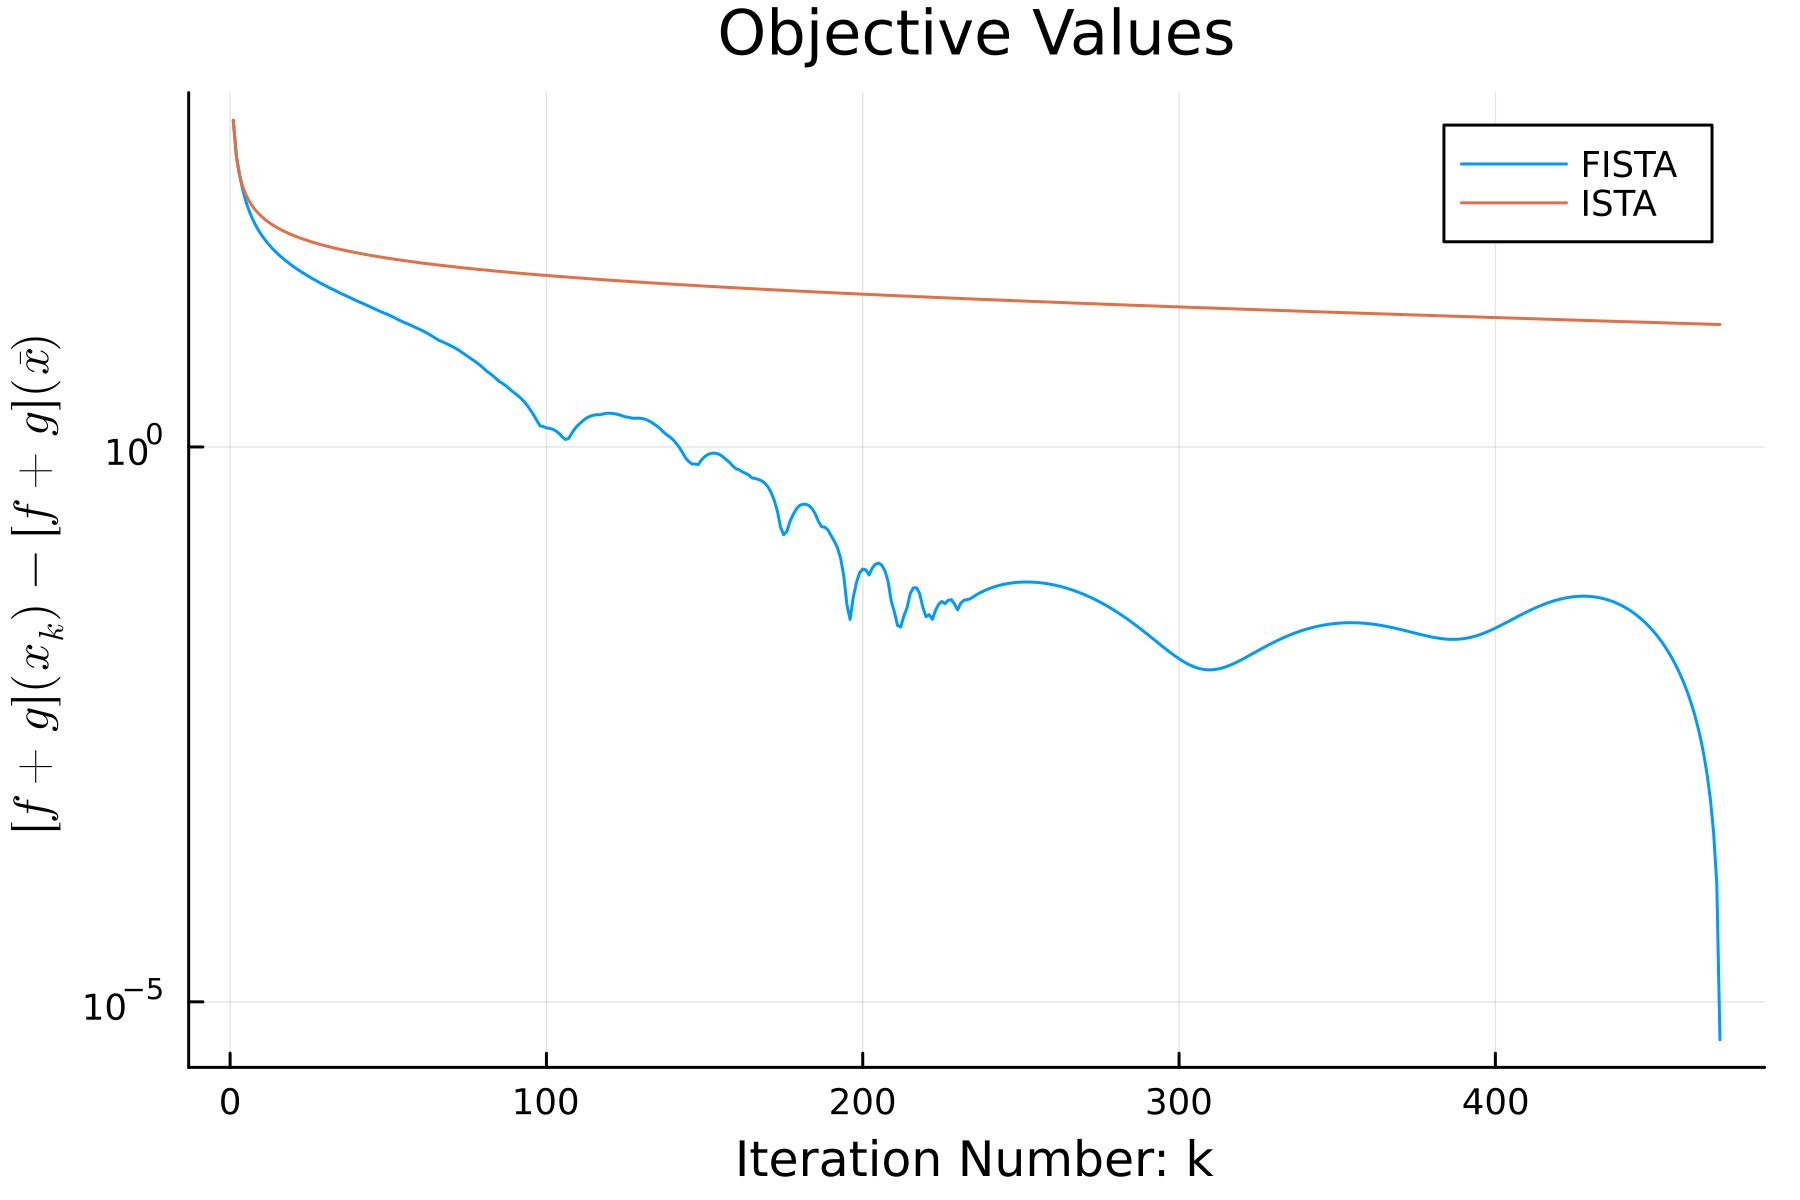
\includegraphics[width=8cm]{simple_lass_obj.png}
                \caption{The left is the objective value of the function during all iterations.}
            \end{figure}
        \end{frame}
        \begin{frame}{Results}
            The plot of $\Vert y^{(k)} - x^{(k + 1)}\Vert_\infty$:
            \begin{figure}[h]
                \centering
                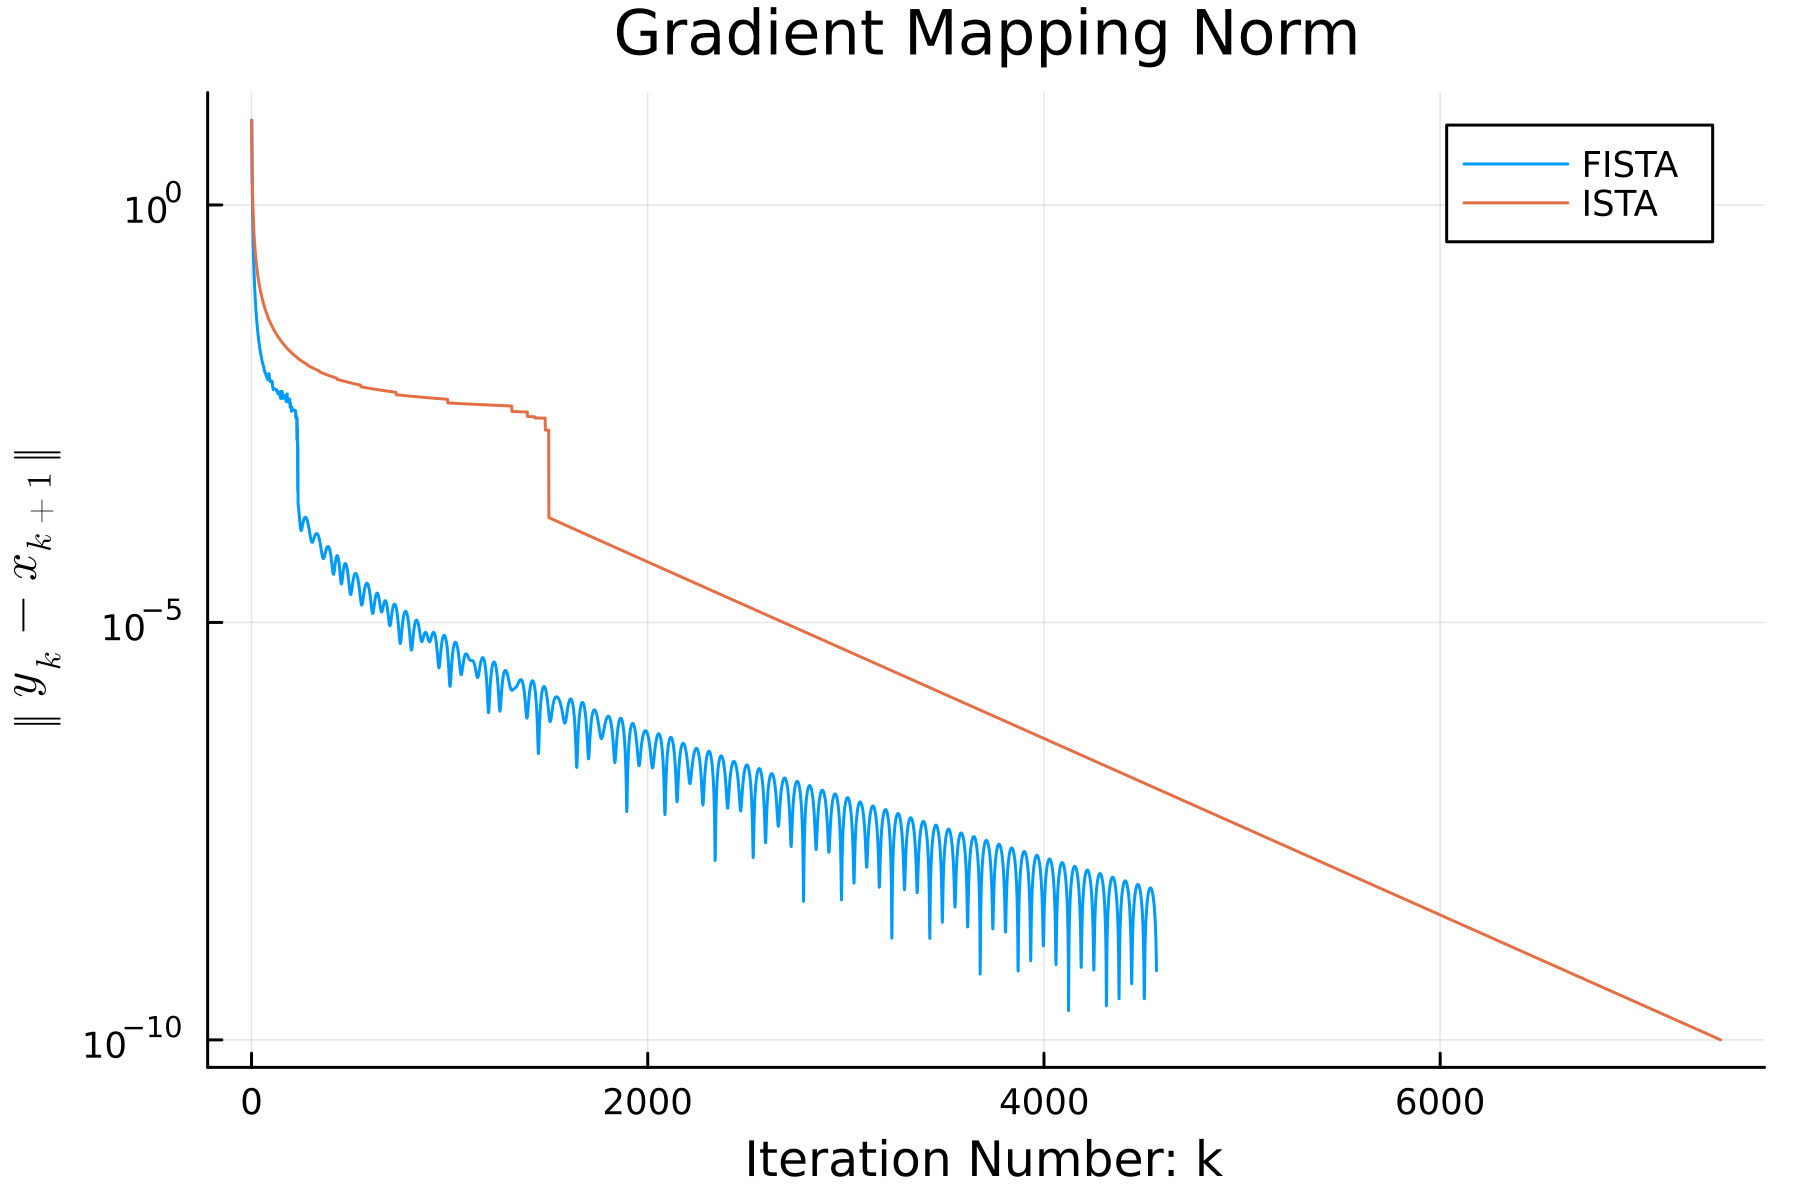
\includegraphics[width=8cm]{simple_lass_pgrad.png}
            \end{figure}
        \end{frame}
    \subsection{Image Deconvolution with Noise}
        \begin{frame}{Experiment Setup}
            Given an image that is convoluted by a Guassian kernel with some guassian noise, we want to recover the image, given the parameters for convolutions. 
            \begin{itemize}
                \item [1.] Guassian blur with a discrete 15 by 15 kernel is a linear transform represented by a sparse matrix $A$ in the computer. 
                \item [2.] When an image is 500 by 500 with 3 color channels, $A$ is $750000 \times 750000$. 
                \item [3.] Let the noise be on all normalized colors values with $N(0, 10^{-2})$
                \item [4.] We let $\lambda = \alpha\times (3\times500^2)^{-1}$. 
                \item [5.] Implemented in Julia, and the code is too long to be shown here. 
            \end{itemize}        
        \end{frame}
        \begin{frame}{The Blurred Image}
            We consider blurring the image of a pink unicorn that I own. 
            \begin{figure}[H]
                \centering
                
\includegraphics[width=5cm]{blurred_img.jpg}
                \caption{The image is blurred by the Gaussian Blurred matrix $A$ with a tiny amount of noise on the level of $2\times 10^{-2}$ that is barely observable. Zoom in to observe the tiny amount of Gaussian noise on top of the blur.}
                \label{fig:blurred_alto}
            \end{figure}
        \end{frame}
        \begin{frame}{Results}
            \begin{figure}[H]
                \centering
                \begin{subfigure}{3.5cm}
                    
\includegraphics[width=3cm]{inverse_linear_experiment1-soln_img.jpg}
                    \caption{} \label{fig:1a}
                \end{subfigure}     %
                % \hspace*{\fill}     % maximize separation between the subfigures
                \begin{subfigure}{3.5cm}
                    
\includegraphics[width=3cm]{inverse_linear_experiment2-soln_img.jpg}
                    \caption{} \label{fig:1b}
                \end{subfigure}     %
                % \hspace*{\fill}     % maximize separation between the subfigures
                \begin{subfigure}{3.5cm}
                    
\includegraphics[width=3cm]{inverse_linear_experiment3-soln_img.jpg}
                    \caption{} \label{fig:1c}
                \end{subfigure}
                \caption{(a) $\alpha = 0$, without any one norm penalty, is not robust to the additional noise. (b) $\alpha = 0.01$, there is a tiny amount of $\lambda$. (c) $\alpha = 0.1$, it is more penalty compared to (a).}
                \label{fig:alto_deblurred}
            \end{figure}
        \end{frame}
        
   
\section{Conclusion}
    \begin{frame}{Contributions}
        \begin{block}{The Paper's Contribution}
            Beck's contribution involves proving that the Nesterov accelerations work for the proximal gradient method. Beck popularized the use of momentum in the broader context to improve the convergence of algorithms such as the proximal gradient method.    
        \end{block}
        \begin{block}{My Contribution}
            I wrote the same proof in a different way for Proximal gradient in both the accelerated case and the unaccelerated case. I avoided using the assumption of Nesterov Momentum term and instead used a template method and the idea of form match to derive the sequence in the middle of the convergence proof.     
        \end{block}
    \end{frame}
    
\section{References}
    \begin{frame}{References}
        
        \bibliography{refs.bib}
    \end{frame}

\end{document}